\chapter{Desenvolvimento \textit{MapReduce}}
\label{cap:mapreduce-devel}

Neste capítulo, discute-se sobre a construção de aplicações baseadas no modelo \textit{MapReduce}. Anteriormente, foi apresentada uma introdução a este novo paradigma, porém o foco desta seção é deixar claro quais são os passos necessários para o desenvolvimento neste ambiente. Será utilizada uma abordagem técnica para descrever os recursos disponibilizados por este \textit{framework}, originalmente criado para linguagem Java. O manual de instalação do \textit{plugin} Hadoop para a ferramenta Eclipse\footnote{\url{http://eclipse.org/}} pode ser encontrado no apêndice \ref{apd-eclipse}.

Hadoop provê uma API para \textit{MapReduce} que permite a construção das funções \textit{map} e \textit{reduce} em outras linguagens de programação \cite{white2012}. É possível realizar o desenvolvimento de aplicações \textit{MapReduce} em linguagens de \textit{script}, por exemplo, Python e Ruby, usando o utilitário \textit{Hadoop Stream}. Para a implementação em C++, utiliza-se uma interface denominada \textit{Hadoop Pipe}.

De acordo com a pesquisa realizada por \citeonline{ding2011}, a implementação em outras linguagens pode ocasionar uma perda de performance, pois a chamada do programa ocasiona \textit{overhead}. Porém quando um job necessita de alto trabalho computacional o uso de linguagens mais eficientes que Java pode trazer benefícios no tempo de execução. O foco deste capítulo será na implementação do \textit{MapReduce} para a linguagem Java.

Para demonstrar sua implementação, será utilizado o exemplo do contador de palavras, também abordado na seção \ref{sec-wc}. Este problema consiste em realizar a contagem de ocorrências das diferentes palavras que aparecem ao longo de um arquivo de texto. Primeiramente será adotada uma solução convencional para sua resolução, posteriormente esta abordagem será adaptada para o modelo \textit{MapReduce}.

A implementação para este contador de palavras pode ser realizada de diversas maneiras. Um algoritmo que pode ser usado para solucionar esta questão é mostrado no quadro \ref{cod-wc-hash}.

A construção deste algoritmo consiste na utilização de um \textit{HashMap\footnote{\url{http://docs.oracle.com/javase/7/docs/api/java/util/HashMap.html}}} para relacionar cada String encontrada a um valor inteiro, incrementado a cada ocorrência no texto, representando sua frequência. A utilização desta estrutura de dados permite uma simples implementação, entretanto para análise de arquivos em larga escala esta estratégia convencional pode se tornar inviável.

A classe \textit{HashMap} compõe uma das implementações da interface \textit{Map}, que por sua vez faz parte dos tipos de coleções disponibilizados pela linguagem Java. O aumento excessivo da quantidade de elementos desta estrutura pode elevar significativamente o uso de memória e também ocasionar uma brusca queda de performance \cite{oaks2014}.

\lstinputlisting[float,
		frame=single,
		breaklines=true,
		label=cod-wc-hash,
		style=java,
		caption={[Algoritmo convencional para contador de palavras]
		Algoritmo convencional para contador de palavras
		\protect\linebreak Fonte: Autor}]
		{quadros/wordcount-hash}

A solução adequada para o contexto Big Data, na qual são analisados arquivos extremamente volumosos, consiste na construção de um algoritmo baseado em computação distribuída. A grande vantagem de utilizar o modelo \textit{MapReduce} é que o desenvolvedor precisa apenas adaptar o problema para ser resolvido com as funções \textit{map} e \textit{reduce}. Toda a complexidade envolvida em paralelizar o processamento é realizada pelo \textit{framework}.

O \textit{MapReduce} é um paradigma que permite uma implementação flexível e simples para esta situação, para tal é necessário apenas três coisas: Uma função \textit{map}, uma função \textit{reduce} e um pedaço de código para execução do \textit{job} \cite{white2012}. Na tabela \ref{tab-mapreduce-job} estão as atividades que ocorrem em um \textit{MapReduce} \textit{job} e quem é o responsável por cada uma delas.

\begin{table}[!ht]
\begin{center}
  \begin{tabular}{|p{5cm}|p{5cm}|}
	\hline
	Atividade & Responsável	
	\\ \hline
	Configurar \textit{Job} & Desenvolvedor
	\\ \hline
	Dividir arquivos de entrada em \textit{input splits} & Hadoop \textit{Framework}
	\\ \hline
	Iniciar \textit{map tasks} com seus respectivos \textit{input splits} & Hadoop \textit{Framework}
	\\ \hline
	Definir função \textit{map} utilizada pelas \textit{map tasks} & Desenvolvedor
	\\ \hline
	\textit{Shuffle}, onde as saídas de cada \textit{map task} são divididas e ordenadas & Hadoop \textit{Framework}
	\\ \hline
	\textit{Sort}, onde os valores de cada uma das chaves geradas pelas \textit{map tasks} são agrupados & Hadoop \textit{Framework}
	\\ \hline
	Iniciar \textit{reduce tasks} com suas respectivas entradas & Hadoop \textit{Framework}
	\\ \hline
	Definir função \textit{reduce}, na qual é chamada uma vez para cada chave existente & Desenvolvedor
	\\ \hline
	Escrever os resultados das \textit{reduce tasks} em N partes no diretório de saída definido nas configurações do job, onde N é o número de \textit{reduce tasks} & Hadoop \textit{Framework}
	\\ \hline
  \end{tabular}
  \captionsetup{justification=centering}
  \caption[Atividades de um \textit{MapReduce} \textit{job}]{Atividades de um \textit{MapReduce} \textit{job}
  \protect\linebreak Fonte: Adaptado de \cite{venner2009}}
\label{tab-mapreduce-job}
\end{center}
\end{table}
\FloatBarrier

No quadro \ref{cod-wc-hash}, a leitura dos arquivos de entrada é realizada pelo próprio programador, na qual utiliza-se um \textit{BufferedReader} para efetuar o processamento da \textit{stream} dos dados. Para o desenvolvimento no paradigma \textit{MapReduce}, as entradas são obtidas pelo próprio \textit{framework}. O programador deve informar a localização dos arquivos e especificar uma classe que implemente a interface \textit{InputFormat}. 

Desta forma, todas as entradas serão convertidas em \textit{input splits} com pares \textit{\{chave, valor\}} especificados pelo \textit{InputFormat} escolhido. O desenvolvedor pode criar sua própria implementação, porém o Hadoop disponibiliza alguns formatos pré-definidos. Algumas destas classes são apresentados na tabela \ref{tab-inputformat}. Segundo \citeonline{white2012}, por padrão o Hadoop adota a classe \textit{TextInputFormat}, a mesma utilizada pelo exemplo que será apresentado na próxima seção.

\begin{table}[!ht]
\begin{center}
  \begin{tabular}{|p{5cm}|p{5cm}|}
	\hline
	\textit{InputFormat} & Chave / Valor	
	\\ \hline
	\textit{KeyValueTextInputFormat} & Os pares chave/valor são identificados a cada linha, separados por um caractere de tabulação horizontal
	\\ \hline
	\textit{TextInputFormat} & A chave representa o número da linha, enquanto o valor é o respectivo texto
	\\ \hline
	\textit{NLineInputFormat} & Similar ao \textit{TextInputFormat}, porém uma chave pode estar relacionada a N linhas
	\\ \hline
  \end{tabular}
  \captionsetup{justification=centering}
  \caption[\textit{InputFormat} disponibilizados pelo Hadoop]{\textit{InputFormat} disponibilizados pelo Hadoop
  \protect\linebreak Fonte: Adaptado de \cite{venner2009}}
\label{tab-inputformat}
\end{center}
\end{table}
\FloatBarrier

\section{Mapper}

No quadro \ref{cod-mapreduce-google}, foi apresentado um algoritmo para resolver o problema da contagem de palavras de acordo com o paradigma proposto pelo modelo \textit{MapReduce}. O primeiro passo para converter este pseudo código para um programa real consiste na criação da função \textit{map}. De acordo com \citeonline{white2012}, esta função é representada pela classe \textit{Mapper}, na qual deve ser implementado o método abstrato \textit{map}(). No quadro \ref{cod-mapper}, é apresentada uma função \textit{map} para o problema proposto.

\lstinputlisting[frame=single,
		breaklines=true,
		label=cod-mapper,
		style=java,
		caption={[Classe \textit{Mapper}]Classe \textit{Mapper}
		\protect\linebreak Fonte: Autor}]
		{quadros/mapper}

Os parâmetros presentes na assinatura da classe representam os tipos \textit{\{chave, valor\}} de entrada e saída referentes a função \textit{map}. No quadro \ref{cod-mapper}, é possível identificar que as entradas são compostas por uma chave do tipo \textit{LongWritable} e por valores da classe \textit{Text}. Isso significa que cada um dos \textit{input splits} são identificados com um inteiro longo e passados em forma de texto para as funções \textit{map}. As saídas de cada função \textit{map} possuem chaves do tipo \textit{Text} que representam as palavras encontradas em cada \textit{input split}, na qual estão associadas a um valor inteiro \textit{IntWritable} indicando uma ocorrência no texto.

O Hadoop utiliza suas próprias variáveis primitivas, elas foram criadas para maximizar a serialização\footnote{Serialização é a habilidade de converter objetos em memória para uma forma externa em que possa ser transmitida (byte a byte) e recuperada posteriormente \cite{darwin2014}.} dos objetos transmitidos pela rede \cite{white2012}. Os tipos \textit{LongWritable}, \textit{IntWritable} e \textit{Text} representam respectivamente os tipos básicos \textit{Long}, \textit{Integer} e \textit{String}. Segundo \citeonline{white2012}, o mecanismo de serialização disponibilizado pela linguagem Java não é utilizado, pois não atende os seguintes critérios: compacto, rápido, extensível e interoperável.

O Hadoop permite que o desenvolvedor implemente seu próprio tipo primitivo e, para isto, basta criar um objeto que implemente a interface \textit{Writable}. Na maioria das situações isto não é necessário, pois são disponibilizados objetos para \textit{arrays}, mapas, e também para todos os tipos primitivos da linguagem Java (com exceção ao \textit{char}). A figura \ref{fig-writable} ilustra todas as implementações do Hadoop para a interface \textit{Writable}.

\begin{figure}[ht!]
	\centering
	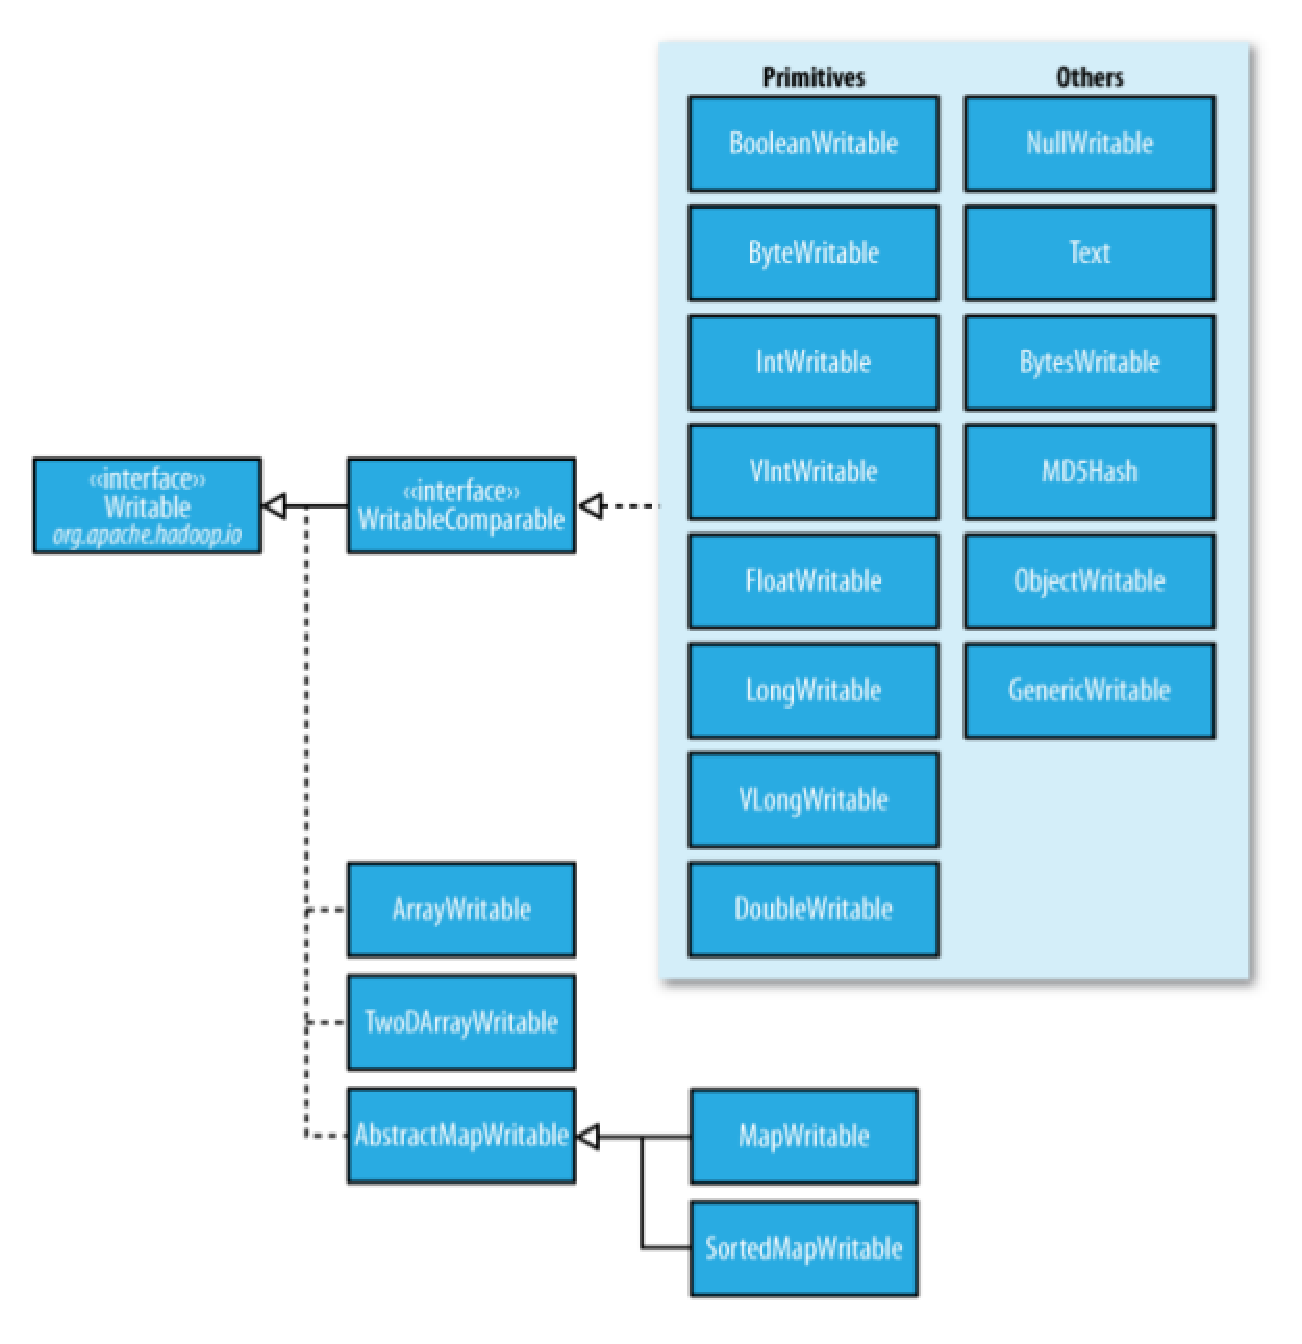
\includegraphics[keepaspectratio=true,scale=0.5]
	  {figuras/hadoop-writable.eps}
	\caption[Hierarquia \textit{Writable}]{Hierarquia \textit{Writable}
	\protect\linebreak Fonte: \cite{white2012}}
	\label{fig-writable}
\end{figure}
\FloatBarrier

A função \textit{map}, definida no quadro \ref{cod-mapper}, é executada para cada \textit{input split} existente. Seus parâmetros representam os pares \textit{\{chave, valor\}} de entrada, e um objeto da classe \textit{Context}, onde os resultados intermediários são armazenados. Dentro da função é possível converter os tipos de dados do Hadoop para os equivalentes em Java, utilizando os recursos disponibilizados pela linguagem normalmente. De acordo com \citeonline{venner2009}, os objetos da classe \textit{Writable} usados para a escrita dos resultados na classe \textit{Context} devem ser reutilizados, evitando a criação de novas instâncias desnecessárias.

\section{Reducer}

A função \textit{reduce} é implementada através da classe \textit{Reducer}, pela qual define-se um método abstrato \textit{reduce}() que deve ser sobrescrito. Assim como a classe \textit{Mapper}, a assinatura de um \textit{Reducer} possui quatros parâmetros indicando os pares \textit{\{chave, valor\}} de entrada e saída. As entradas para a função de redução consistem nos tipos de dados de saída especificados pela função \textit{map}, e também em um objeto da classe \textit{Context}. Assim como na classe \textit{Mapper}, ele será responsável por receber os resultados gerados por esta etapa. 

O primeiro parâmetro da função reduce indica a chave do tipo \textit{Text}, que representa uma palavra encontrada no texto pela função \textit{map}. A próxima entrada é uma lista de valores do tipo \textit{IntWritable} resultante do agrupamento realizado pelas fases \textit{shuffle} e \textit{sort}. A responsabilidade deste método é apenas somar os valores da lista e escrever os resultados da contagem da chave no objeto \textit{Context}. O quadro \ref{cod-reducer} apresenta a implementação da classe \textit{Reducer}.

\lstinputlisting[frame=single,
		breaklines=true,
		label=cod-reducer,
		style=java,
		caption={[Classe \textit{Reducer}]Classe \textit{Reducer}
		\protect\linebreak Fonte: Autor}]
		{quadros/reducer}

Após a leitura do capítulo \ref{cap:hadoop}, fica claro que o \textit{MapReduce} procura otimizar a quantidade de dados que são transmitidos pela rede, desta forma, o ideal é realizar o máximo de operações locais possíveis. As \textit{map tasks} podem gerar uma grande quantidade de resultados intermediários, que posteriormente serão copiados para as máquinas onde são executadas as \textit{reduce tasks}. Muitos destes valores podem ser simplificados antes de serem enviados para a rede. O Hadoop permite que o desenvolvedor especifique uma função chamada \textit{combine} a fim de reduzir as saídas geradas pelas funções \textit{map} \cite{white2012}.

Esta função pode ser interpretada como uma pequena fase \textit{reduce}, que ocorre logo após uma \textit{map task} produzir seus resultados. De acordo com \citeonline{ghemawatMapreduce2008}, em muitas situações o código utilizado para a função \textit{combine} é o mesmo para a função \textit{reduce}. Considere os seguintes resultados gerados por uma \textit{map task} para o exemplo de contagem de palavras:

\begin{lstlisting}[style=abnt,frame=none]
(the, 1)
(the, 1)
(Hadoop, 1)
(Hadoop, 1)
(Hadoop, 1)
(Hadoop, 1)
(framework, 1)
\end{lstlisting}

Ao aplicar a função combine, os resultados gerados são simplificados para:

\begin{lstlisting}[style=abnt,frame=none]
(the, 2)
(Hadoop, 4)
(framework, 1)
\end{lstlisting}

Desta forma, os resultados transmitidos pela rede podem ser reduzidos significativamente. É importante ressaltar que existem situações em que esta abordagem não pode ser aplicada. Para um programa que realize a média aritmética, por exemplo, usar uma função \textit{combine} pode gerar resultados incorretos, pois simplificar valores intermediários resultará em um cálculo impreciso da média de todos os valores. Portanto é necessário analisar o contexto para a aplicação de uma função \textit{combine}.

\section{Configuração do Programa}

O último passo para finalizar a construção do programa \textit{MapReduce} consiste em definir as configurações do \textit{job} e utilizar uma classe principal para executá-lo. A classe \textit{Job} representa o programa \textit{MapReduce} em questão. Através dos métodos \textit{setMapperClass}(), \textit{setCombinerClass}() e \textit{setReducerClass}() é possível especificar as classes utilizadas para as funções \textit{map}, \textit{combine} e \textit{reduce}, respectivamente. A classe \textit{WordCount} apresentada no quadro \ref{cod-job} é responsável pela execução do \textit{job}, assim como especificado pelo método \textit{setJarByClass}().

A localização dos arquivos de entrada, que serão utilizados pelo programa, são indicados pelo método \textit{addInputPath}(). No quadro \ref{cod-wc-hash}, a escrita dos resultados do programa é realizada pelo próprio programador percorrendo os valores do \textit{HashMap}, já no modelo \textit{MapReduce} o desenvolvedor apenas especifica o formato de saída do arquivo através dos métodos \textit{setOutputKeyClass}() e \textit{setOutputValueClass}().

\lstinputlisting[frame=single,
		breaklines=true,
		label=cod-job,
		style=java,
		caption={[Classe para executar \textit{MapReduce job}]Classe para executar \textit{MapReduce job}
		\protect\linebreak Fonte: Autor}]
		{quadros/jobrunner}

Após a execução das reduce tasks, o \textit{framework} será responsável por escrever os resultados registrados no objeto da classe \textit{Context} em um diretório  especificado pelo método \textit{setOutputPath}(). Este ficheiro não deve existir no HDFS, segundo \citeonline{white2012}, isto evita que informações sejam sobrescritas acidentalmente. O método \textit{waitForCompletion}() submete o \textit{job} para ser executado e aguarda o término do processo. O parâmetro booleano indica a escrita das informações do programa no \textit{console} durante a execução.


